\section{Residual Neural Networks}
\label{sec:neural-networks}

\Todo{Maybe use this somehow}A part of the success of neural networks can be explained not only by mathematics but also physics.
It seems to be the case that neural networks are not very cost efficient in approximating any function, but are for most functions humans are interested in.

In \cite{owhadi20}, the author models a special class of neural networks, called Residual Neural Networks (ResNets), and proves their convergence to a known problem, as the number of layers increases towards infinity.
ResNets were first introduced by \citet{he16} in 2016 and have their origins in practical application rather than theory.
This section provides a short introduction to ResNets and what problem they solve.
Some basic knowledge of neural networks is presumed.

In the early 2010s, when neural networks started to become increasingly popular it was still difficult to train models with many layers.
Neural network architectures with many layers ("deep" networks) have led to many breakthroughs in supervised learning tasks.
There is evidence that the number of layers (the depth) is of high importance:
Non-flattening theorems state the the number of neurons required by a shallow network, i.e. one with only one hidden layer, grows (almost) exponentially compared to a deep network \cite{lin17,delalleau11}.
An example: the product of $n$ numbers can be computed by a deep network with only $4n$ neurons, where as a flattened equivalent with only one hidden layer would require $2^n$ neurons \cite{lin17}.

These facts justify the conjecture that the deeper a network is, the better its performance.
The greater number of parameters resulting from added layers should lead to an improvement --  or at least not worsen the results.
\citet{he16} constructed an easy example for a deeper network with the same performance as a shallow one:
Take a trained (shallow) network and copy its parameters to the first layers of the deep network.
Set the remaining layers such that they perform an identity mapping, which means they just pass the input through to the next layer without changing it.
This indicates that in general, a deeper network should not produce worse results than one with fewer layers.

\begin{figure}
	\makebox[\textwidth][c]{
		\centering
		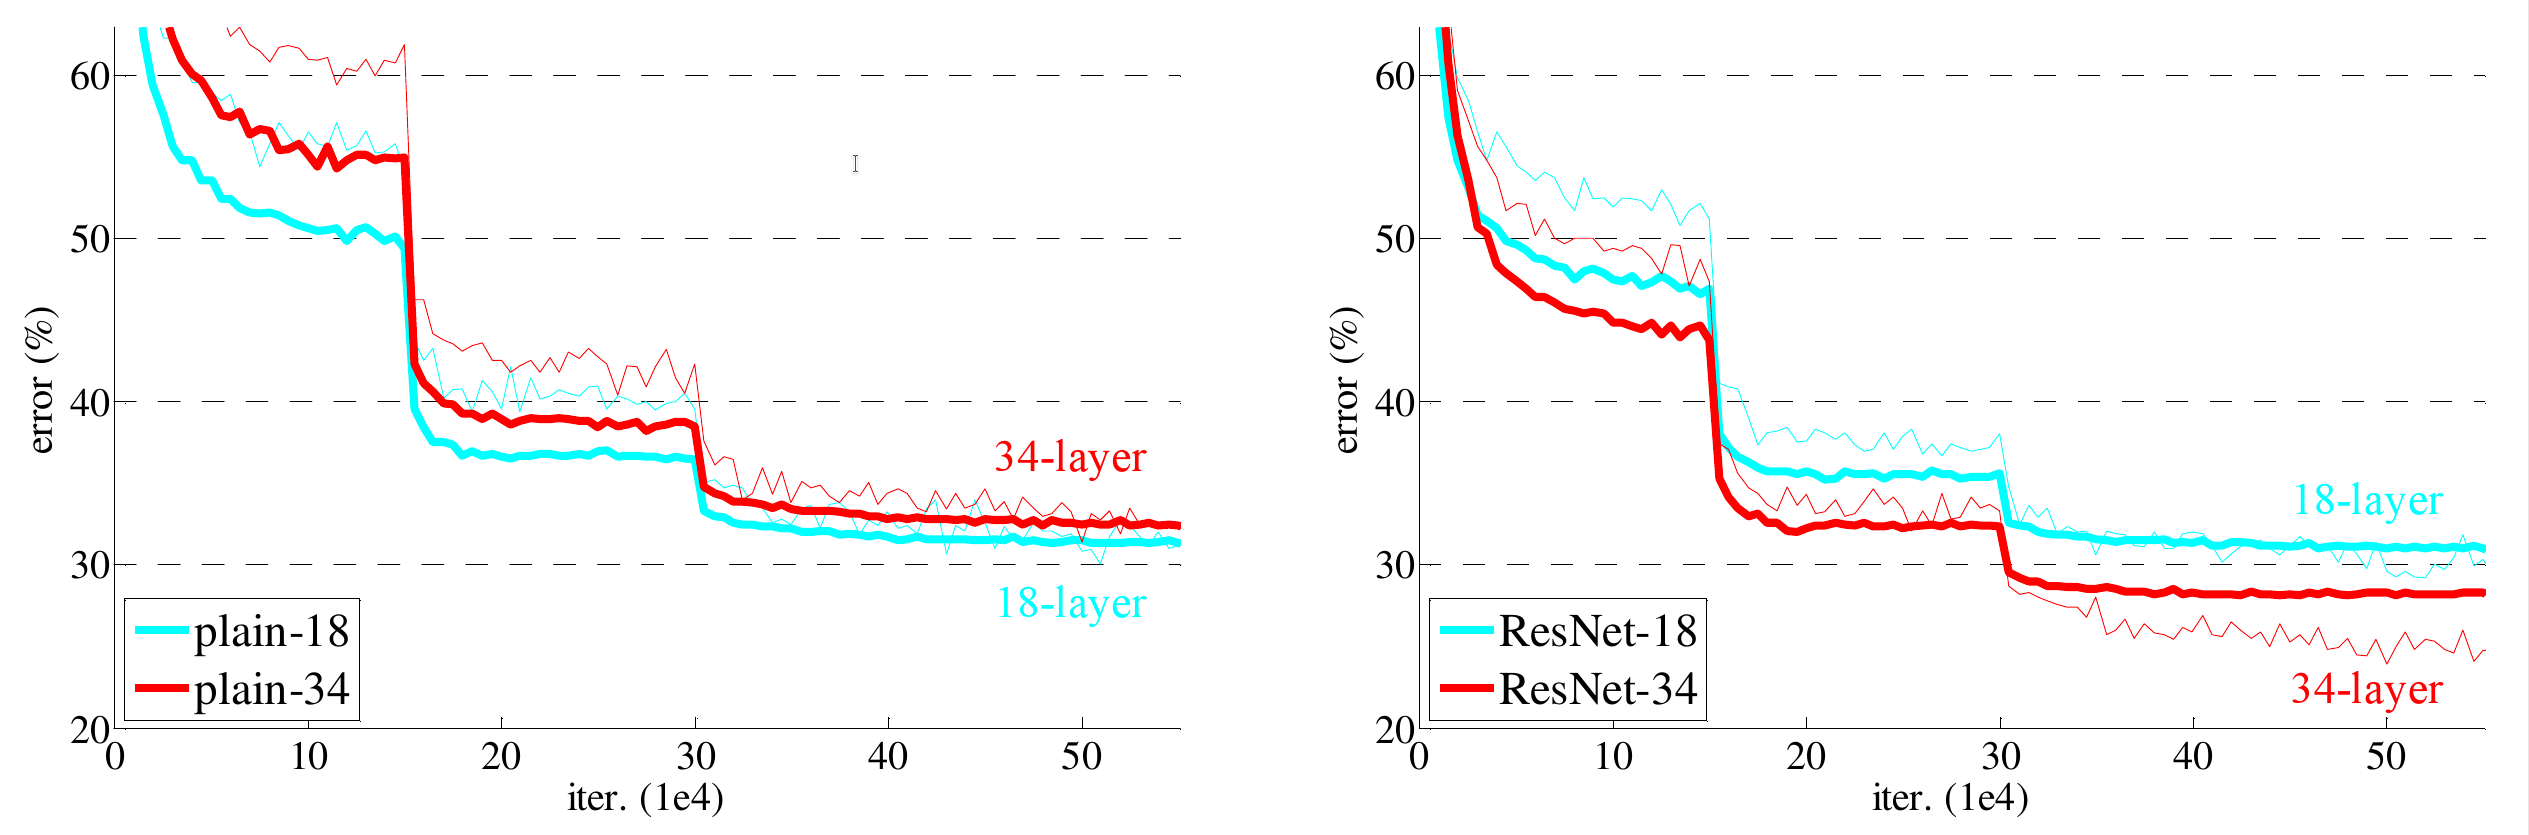
\includegraphics[scale=0.4]{figures/image_net_error_by_kaiming_he.png}
	}
	\caption{
		Training (thin) and validation errors (bold) for a 18- and 34-layer plain network (left) and ResNet (right).
		The plain 34 layer network shows worse results than the 18 layer equivalent, whereas the deeper ResNet performs better than the 18 layer one.
		This is not the case for the plain network.
		This figure originates from the paper "Deep Residual Learning for Image Recognition" by \citet{he16}. \copyright~2016 IEEE.}
	\label{fig:depth-performance-decline}
\end{figure}

Yet in practice one can observe deteriorating performance after a certain depth has been reached.
An example for this can be seen in \cref{fig:depth-performance-decline} on the left.
If the decline was measurable only for the test error it could have been attribute to overfitting, which can happen if the chosen architectures are too complex.
However, in this case the adverse effects are also present for the training error.
It seems that contemporary optimizers are not able to effectively learn the constructed solution from above.
Thus, \citet{he16} conjecture that it is hard to learn the identity mapping through non-linear layers and suggest that it is easier to learn the zero function instead.
This leads to their proposed network architecture: Residual Neural Networks (ResNets).

The characteristic feature of ResNets is that they learn residual mappings instead of unreferenced mappings.
Let $f: \cX \rightarrow \cX$ be the function to be approximated by number of (non-linear) layers and $x \in \cX$.
\citet{he16} suggest that instead of learning $f$ directly, to learn the \emph{residual}; given by
\begin{equation}
	\begin{split}
		g: \cX \rightarrow \cX \\
		g(x) \coloneqq f(x) - x \ .
	\end{split}
\end{equation}
This is implemented by creating shortcut connections that skip one or more layers and add the input to the layers' output, resulting in $g(x) + x = f(x)$.
An illustration of a typical residual block is shown in \cref{fig:residual-block}.

\begin{figure}
	\centering
	\begin{tikzpicture}
		[
		font=\scriptsize,
		block/.style ={rectangle, draw=black, thick, text width=15em, align=center, minimum height=1.5em}
		]
		\node[] (a) [block] {Fully Connected Layer (1024)};
		\node[below= -1.5\pgflinewidth of a] (a1) [block] {BatchNorm};
		\node[below= -1.5\pgflinewidth of a1] (b) [block] {ReLU};
		\node[below= 4mm of b] (c) [block] {Fully Connected Layer (1024)};
		\node[below= -1.5\pgflinewidth of c] (c1) [block] {BatchNorm};
		\node[below= -1.5\pgflinewidth of c1] (d) [block] {ReLU};
		\node[below= 4mm of d] (e) [block] {$\bigoplus$};
		\node[above=of a] (x) [] {};
		\draw[->, line width=1pt] (b.south) -- (c.north);
		\draw[->, line width=1pt] (d.south) -- (e.north);
		\draw[->, line width=1pt] (x) -- (a);
		\node[below=of e] (y) [] {};
		\draw[->, line width=1pt] (e) -- (y);
		\node[above=.4 of a] (z) [] {};
		\node[right=12em of z] (h) [] {};
		\draw[line width=1pt] (z.center) -- (h.center);
		\draw[->, bend right, line width=1pt] (h.center) |- (e.east);
	\end{tikzpicture}
	\caption{Typical residual block.
	$\bigoplus$ indicates the inputs of both arrows being summed.
	This particular design was used in \cite{drover18} for 3D Human Pose Estimation.
	Similar blocks are used in image classification and object detection, where the fully connected layers are usually replaced by convolutions.
	}
	\label{fig:residual-block}
\end{figure}

This residual network layout was able to circumvent the decrease in performance that came with an increased number of layers and even showed better results, as one would expect from a model with a greater number of parameters.
Nowadays, ResNets are used in virtually all areas of machine learning, including image classification and object detection \cite{he16}, semantic segmentation \cite{chen17}, 3D human pose estimation \cite{drover18} and natural language processing \cite{keskar19,conneau16}.
